\section{Casos de uso}

Para comprobar el correcto funcionamiento del sistema desarrollado, hemos establecido una serie de casos de prueba representativos que se muestran a continuación:






Hemos elegido dividirlos en tres grupos:
\begin{enumerate}
	\item El enemigo no sobrevive al ataque.
	\item El enemigo sobrevive al ataque pero nuestro personaje no.
	\item El enemigo sobrevive y nuestro personaje también.
\end{enumerate}

\begin{enumerate}

	\item En el primer grupo, hemos elegido dos casos representativos, uno de los cuales se subdivide:
	\begin{enumerate}[label={1.\arabic*.}]
		\item La precisión es media-alta. Teniendo esto en cuenta, es fácil decidir que lo mejor es atacar, ya que el enemigo es muy probable que no sobreviva al ataque y por tanto el combate terminaría en una victoria. Como se puede observar en la tabla, el sistema devuelve un resultado coherente con el anterior razonamiento, dándole al Ataque una adecuación del 0,915, mientras que a Curación y Defensa sólamente un 0,189.
		\item La precisión es baja. En este caso debemos fijarnos en si el personaje sobreviviría o no al fallar el ataque, por lo que dividimos este caso en dos subcasos:
		\begin{enumerate}[label=\alph*)]
			\item El personaje sobrevive. Sabiendo esto, debemos comprobar la vida restante al defenderse y al curarse. Si suponen una mejora lo suficientemente importante, la Curación o la Defensa tendrán más adecuación que el Ataque. Se puede observar que los resultados arrojados por el sistema son coherentes.
			\item El personaje no sobrevive. Como es lógico, en este caso debemos pensar en Curación y Defensa como las opciones más viables y optar por una o la otra en función de la vida restante al realizar cada una de ellas. De nuevo, el sistema devuelve unos resultados razonables.
		\end{enumerate}
	\end{enumerate}
\item[] \begin{figure}[H]
	\centering
	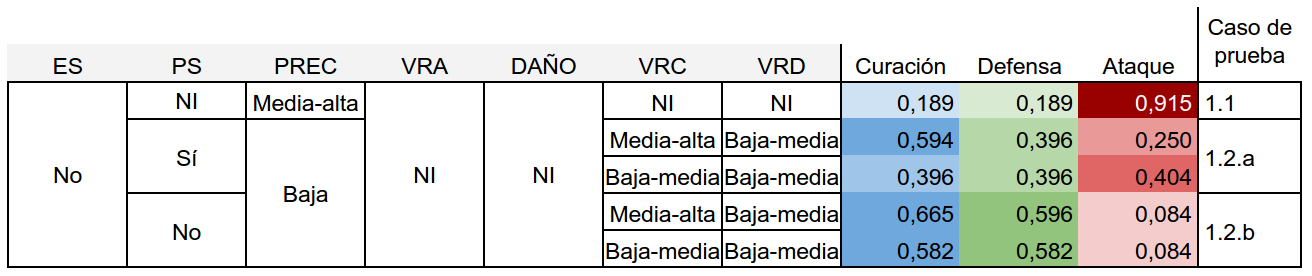
\includegraphics[width=\textwidth,height=\textheight,keepaspectratio]{images/casos_pruebas.png}
	\caption{Casos de prueba 1}
	\label{fig:casos_prueba1}
\end{figure}

\item[] \begin{figure}[H]
	\centering
	\includegraphics[width=\textwidth,height=\textheight,keepaspectratio]{images/ejecución_1_2_a.png}
	\caption{Ejemplo de ejecución para el caso de uso 1.2.a}
	\label{fig:casos_prueba1}
\end{figure}

\item El segundo grupo se asemeja al caso 1.2.b del primer grupo. Nuestro personaje no sobrevive al ataque, por lo que debe centrarse en Curación o Defensa. Igual que en el 2.b, debemos decidir en función de la vida restante, y seguimos obteniendo resultados lógicos.

\item[]
\begin{figure}[H]
	\centering
	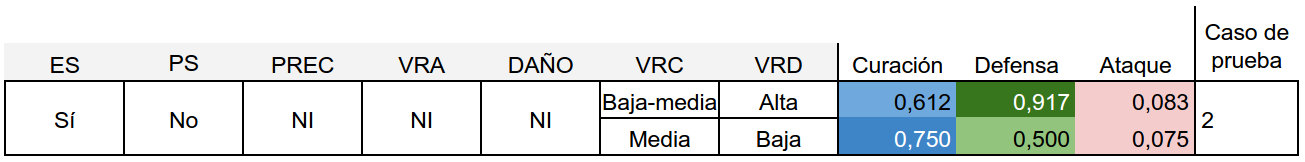
\includegraphics[width=\textwidth,height=\textheight,keepaspectratio]{images/casos_pruebas1.png}
	\caption{Casos de prueba 2}
	\label{fig:casos_prueba2}
\end{figure}

\item[] \begin{figure}[H]
	\centering
	\includegraphics[width=\textwidth,height=\textheight,keepaspectratio]{images/ejecución_2.png}
	\caption{Ejemplo de ejecución para el caso de uso 2}
	\label{fig:casos_prueba1}
\end{figure}

\item El último grupo es algo más complicado, ya que se deben tener en cuenta más factores para poder realizar una acción óptima, como el daño que vamos a realizar y la vida restante después de realizar un ataque. Podemos distinguir dos casos representativos, que a su vez se dividen en subcasos:
\begin{enumerate}[label={3.\arabic*.}]
	\item La vida restante del personaje después de atacar es media-alta. Podemos centrarnos ahora en decidir con cuánta adecuación atacamos, ya que la Curación y Defensa nos privarían de una buena oportunidad para atacar:
	\begin{enumerate}[label=\alph*)]
		\item La precisión es media-alta. Para tener un mejor criterio, nos ayudamos de la variable de entrada DAÑO. Con un daño medio-alto, la adecuación del Ataque debe ser muy alta y la de Curación y Defensa muy baja. Con un daño bajo, el Ataque seguiría siendo una buena opción aunque con peor adecuación. Los resultados al establecer estos datos en el sistema, concuerdan con el razonamiento que hemos llevado a cabo.
		\item La precisión es baja. En este caso no es necesario tener en cuenta ninguna otra variable. El Ataque es medianamente adecuado y la Curación y Defensa deben ganar algo de adecuación, aunque sin superar el Ataque. Como podemos observar, los datos obtenidos vuelven a ser razonables.
	\end{enumerate}
	\item La vida restante del personaje después de atacar es baja. Debemos tener cuidado, por lo que decidimos la adecuación de las tres opciones en función de la vida restante después de curarse y después de defenderse. Si ambas son tan bajas como la vida restante después de atacar, el ataque es la mejor opción. Sin embargo, en caso contrario, la adecuación será mayor para Curarse o Defenderse, dependiendo de la cantidad de vida restante en cada caso. Los resultados del sistema siguen, de nuevo, el razonamiento llevado a cabo.
\end{enumerate}


\begin{figure}[H]
	\centering
	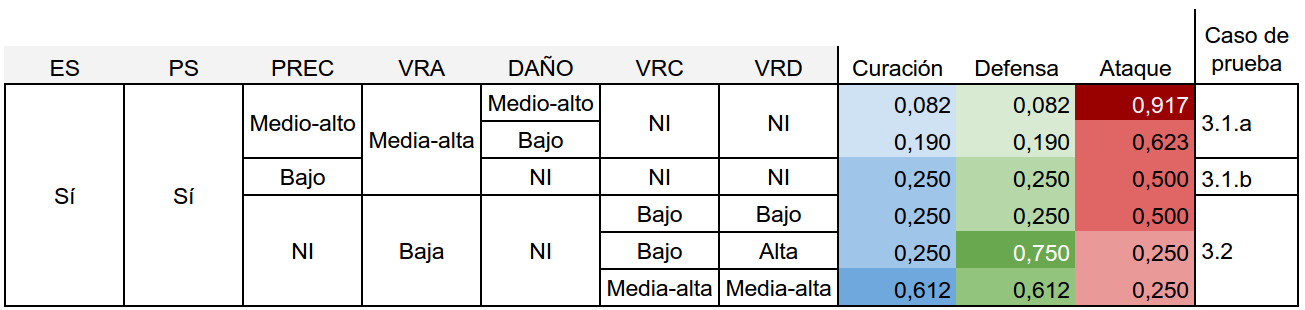
\includegraphics[width=\textwidth,height=\textheight,keepaspectratio]{images/casos_pruebas2.png}
	\caption{Casos de prueba 3}
	\label{fig:casos_prueba3}
\end{figure}

\item[] \begin{figure}[H]
	\centering
	\includegraphics[width=\textwidth,height=\textheight,keepaspectratio]{images/ejecución_3_1_a.png}
	\caption{Ejemplo de ejecución para el caso de uso 3.1.a}
	\label{fig:casos_prueba1}
\end{figure}

\end{enumerate}